\section{Modelling Previous Design}\label{sec:old-design-method}
Because microgravity is incredibly costly to achieve experimentally, a numerical investigation of the old design was conducted using Ansys Fluent. The simulation was ran once with gravity and once without to compare the distribution of powder within the tank and the mass flow rate. 

Initially, an axisymmetric simulation using square cells of 0.4mm was attempted. The axisymmetric configuration was chosen as it would have ran as fast as a 2D simulation, because of the reduced number of cells, while maintaining the 3D physics of the real system. It is assumed the fineness of the mesh used allowed for strong gradients in flow conditions to be resolved as the simulation was numerically unstable and repeatedly crashed. To solve this a new 2D simulation with a coarser mesh of 1mm square cells was conducted, seen in \autoref{fig:old-design-sim}.
\begin{figure}[htbp]
    \centering

    \begin{minipage}{0.3\textwidth}
        \centering
        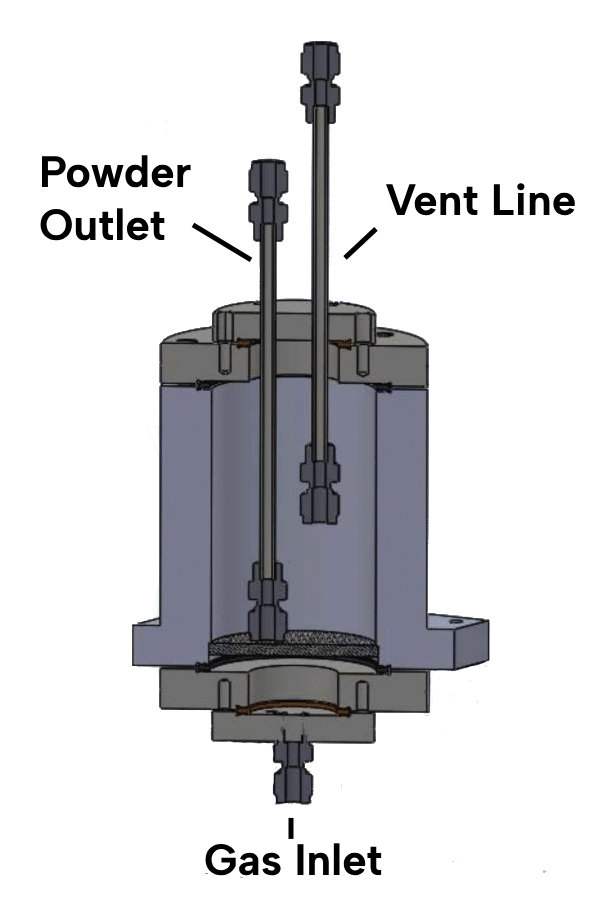
\includegraphics[width=\textwidth]{../report_assets/COSMOS_DIAGRAM_2x3.png}
        \caption*{(a) Previous Design}
    \end{minipage}
    \hfill
    \begin{minipage}{0.3\textwidth}
        \centering
        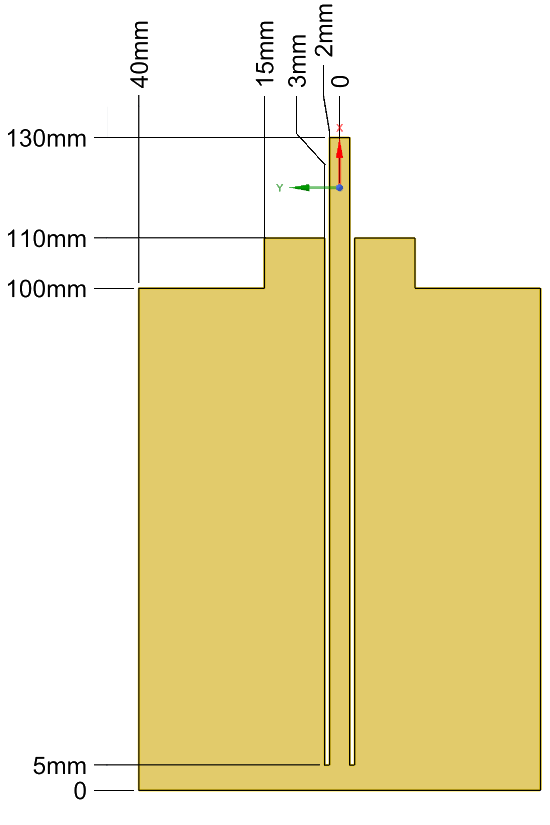
\includegraphics[width=\textwidth]{../report_assets/geom_old.png}
        \caption*{(b) Simplified Geometry}\label{fig:idkyet9}
    \end{minipage}
    \hfill
    \begin{minipage}{0.3\textwidth}
        \centering
        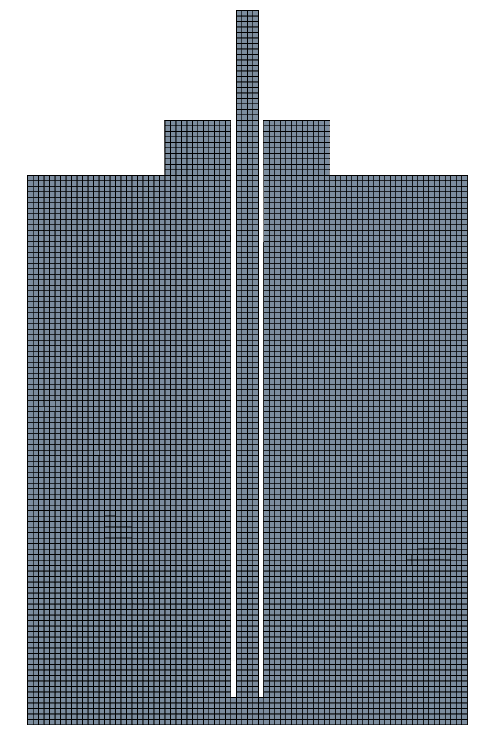
\includegraphics[width=\textwidth]{../report_assets/mesh_old.png}
        \caption*{(c) Mesh Used for Sim}\label{fig:idkyet10}
    \end{minipage}
    
\end{figure}\label{fig:old-design-sim}
While the 2D nature of the simulation means the quantities like mass flow rate or inlet conditions can not be matched to the real system, the key flow characteristics of interest are still expected to remain. This is because particle position within the tank and fluidisation are not reliant on 3 dimensions. A simplified geometry, seen in \autoref{fig:old-design-sim} (b), was used as it sped up computational time while still preserving the geometric features of interest. It is important to note that the vent line pipe was omitted and the outlet pipe was moved to the center, neither of these are expected to impact on the behaviour being investigated. The bottom of the tank held the wire mesh on which the powder sat and represents the bottom of the geometric surface. In the simulation it acted as the velocity inlet in which gas entered the system at a velocity of 0.1m/s. To simulate the two gas and powder phases, a eulerian-eulerian model was used with a gidaspow drag model as this has been shown to best represent fluidising beds~\cite{C6RA28615A}. The powder was modelled as TI6AL4V as this was used during the COSMOS project. Titanium alloy powder used in SLS printing has a particle size distribution between $15\,\mu\mathrm{m}$ and $53\,\mu\mathrm{m}$ and a density between $2.04\ \mathrm{g/cm^3}$ and $2.34\ \mathrm{g/cm^3}$~\cite{ma17040952}, which is assumed to be similar to the powder used in CSAM.\@ Hence a $40\,\mu\mathrm{m}$ particle size and $2200\ \mathrm{kg/m^3}$ density was used. The gas was modelled as nitrogen at standard operating conditions as this was also used during the COSMOS project.

\section{Choosing A New Feed System Architecture}\label{sec:system_architecture}
As discussed in \autoref{sec:prev-design-analysis}, the results of the analysis into the previous design supported the hypothesised issues. Therefore, a new design was desirable and research into current powder feed technology was conducted to better understand the strengths and weaknesses of prior systems. A thorough review of analogous systems was conducted, however it is a possibility that key papers may have been overlooked. The only research paper found on powder-based AM experiments conducted in microgravity originate from the Fraunhofer Institute for Transportation and Automation Technology. Yet, this report offers scant details on the powder-feed mechanism employed~\cite{OVERMEYER2025}. 

Accordingly, five common terrestrial powder-dispensing methods were examined, comparing both their efficacy in the space environment without modifications and the difficulty of implementing the changes required. Only basic schematics of these methods are presented in \autoref{fig:powder-dispensing-methods} as the details for the unchosen architectures is not relevant and the chosen architecture is outlined in \autoref{sec:fluidised-powder-feed-systems}. 
\begin{figure}[htbp]
    \centering

    % First row: 3 images
    \begin{minipage}{0.3\textwidth}
        \centering
        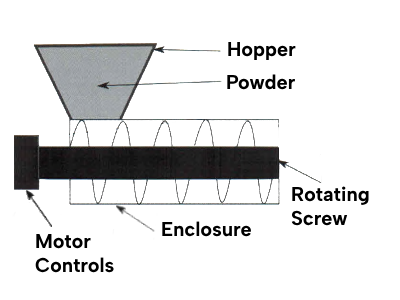
\includegraphics[width=\textwidth]{../report_assets/screw_feed_polished.png}
        \caption*{(a) Screw Fed Design~\cite{Bitragunta2015}}
    \end{minipage}
    \hfill
    \begin{minipage}{0.3\textwidth}
        \centering
        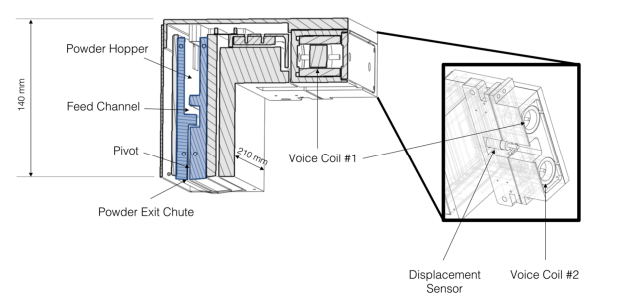
\includegraphics[width=\textwidth]{../report_assets/vibrational_feed.png}
        \caption*{(b) Vibration Fed Design~\cite{Sinclair2021}}
    \end{minipage}
    \hfill
    \begin{minipage}{0.3\textwidth}
        \centering
        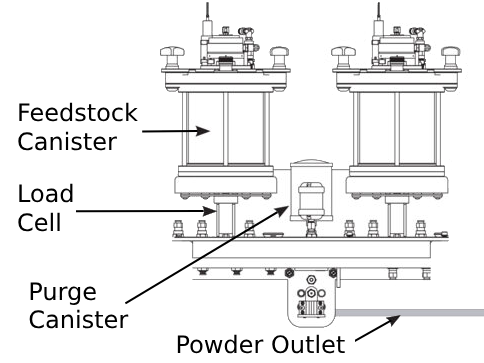
\includegraphics[width=\textwidth]{../report_assets/Liquid_oerlikon.png}
        \caption*{(c) Liquid Suspension Design~\cite{OerlikonMetcoFeeders2023}}
    \end{minipage}

    \vspace{0.5cm} % space between top and bottom rows
    
    % Second row: 2 images
    \begin{minipage}{0.35\textwidth}
        \centering
        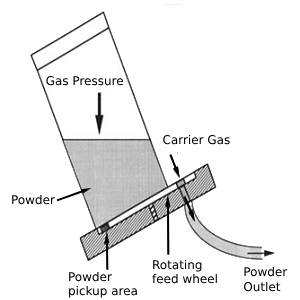
\includegraphics[width=\textwidth]{../report_assets/rotating_disk.png}
        \caption*{(d) Rotating Disk Design~\cite{Crawmer2013}}
    \end{minipage}
    \hspace{0.1\textwidth}
    \begin{minipage}{0.35\textwidth}
        \centering
        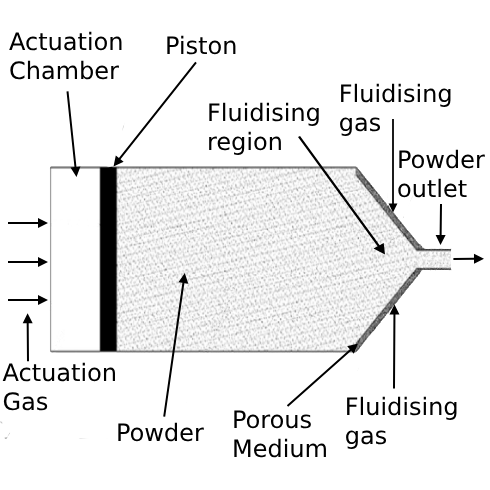
\includegraphics[width=\textwidth]{../report_assets/fluidising_powder_design.png}
        \caption*{(e) Fluidised Powder Bed Design~\cite{Li2016}}
    \end{minipage}
    
    \caption{5 Common Powder Feed System Architectures}\label{fig:powder-dispensing-methods}
\end{figure}
The tabulation of the full analysis can be found in \autoref{appendix:feed-architecture-analysis}. Given that CSAM requires an accelerant gas, the fludising powder bed design was chosen as the most promising design as it mitigates one of the architectures largest drawbacks. Furthermore, the method is assumed to be less affected by microgravity than other options as the main forces the particle experiences are fluid mechanical in nautre, requiring no adjustments of the core mechanic of feeding. 

As mentioned in \autoref{sec:fluidised-powder-feed-systems}, the fluidising powder bed architecture has gone through a number of design iterations since it's first implementation due to miniaturisation. To align the investigation with state-of-the-art systems, the pneumatically driven, permiable piston architecture was chosen. 

\section{Hopper Tank Design}
In fluidised powder feed systems, the tank serves a dual purpose. When not in operations, it acts as a storage vessel, securely holding the powder in a fluidisable state. During operations, the same tank functions as a delivery mechanism, enabling the controlled dispensing of powder through actuation of the piston and the introduction of fluidising gas. 

From previous experience operating the CSAM system used in the COSMOS project, successful samples were produced with inlet pressures between 5 to 8 bar. Therefore, 8 bar was chosen as the designed operating pressure for the tank. It is expected that this subsystem will see pressure lower than or equal to the rest of the system would be able to facilitate tests with an inlet pressure of 8 bar. Though the standard safety factor for pressure vessels is 3.5 - 4~\cite{redriver2024asme}, this was not known at the time of design and only after manufacturing it was discovered. In future iterations, this would be adjusted for by thickening the tank walls as well as using radial bolts for the outlet end cap to tube connection.

The end caps were manufactured from Acetal C POM Delrin as the material is low-cost, easy to machine and chemically inert. The tube was made from clear acrylic to allow the flow behaviour to be observed. Upon evaluation, polycarbonate would have been more appropriate as it is less prone to shattering~\cite{SADEGHIESFAHLANI2021e06856}.
\begin{figure}[htbp]
    \centering

    \begin{minipage}{0.3\textwidth}
        \centering
        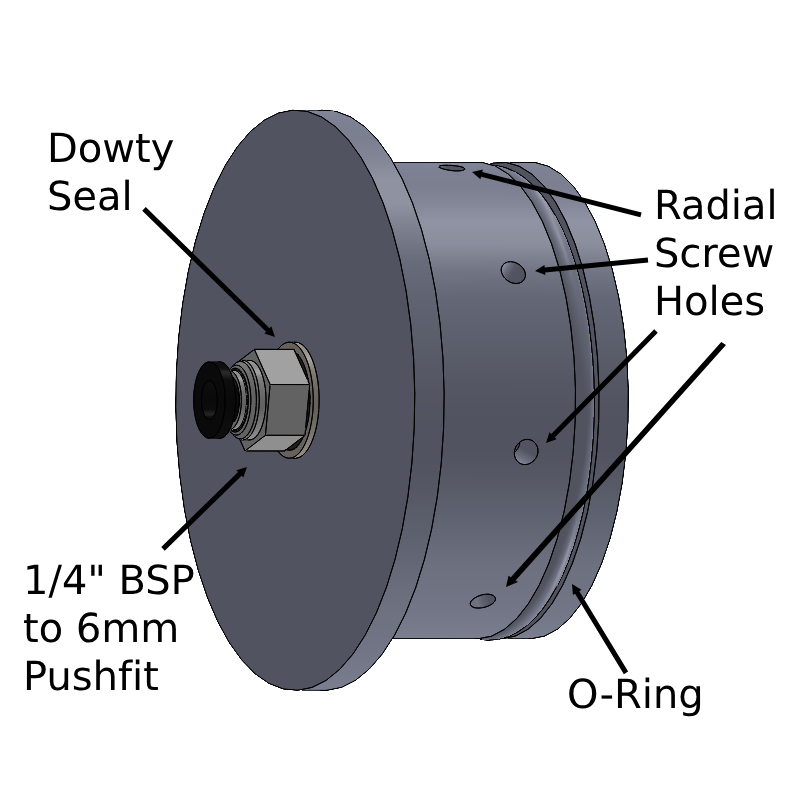
\includegraphics[width=\textwidth]{../report_assets/inlet_end_cap.png}
        \caption*{(a) Inlet End Cap}
    \end{minipage}
    \hfill
    \begin{minipage}{0.3\textwidth}
        \centering
        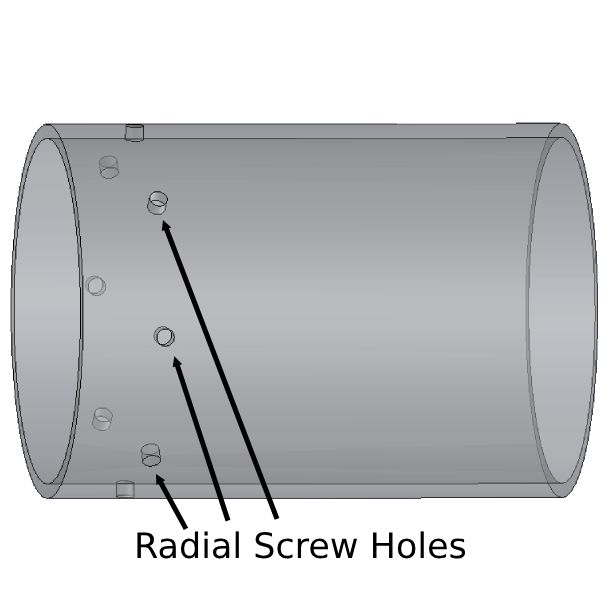
\includegraphics[width=\textwidth]{../report_assets/tube.png}
        \caption*{(b) Acrylic Tube}
    \end{minipage}
    \hfill
    \begin{minipage}{0.3\textwidth}
        \centering
        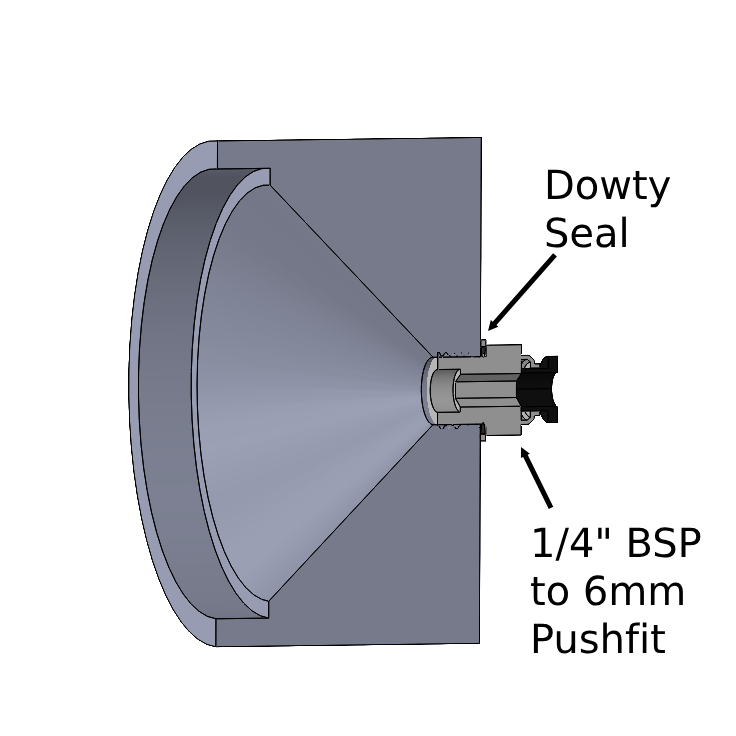
\includegraphics[width=\textwidth]{../report_assets/outlet_end_cap.png}
        \caption*{(c) Outlet End Cap Cross Section}
    \end{minipage}
    \caption{Components of the Hopper Tank}\label{fig:hopper-tank-components}
\end{figure}
As seen in \autoref{fig:hopper-tank-components}, the inlet end cap is radially screwed into the tube. This was done as one of the end caps had to be removable to allow for testing different piston designs. The outlet end cap was bonded to the tube using plastic-friendly epoxy.
\section{Hopper Tank Analysis}
To validate that the design could operate at a pressure of 8 bar, a combination of hand calculations and finite element analysis (FEA) using solidworks was conducted. The failure modes analysed were stress concentrations from the bolt holes and hoop stress rupture. Fracturing at the delrin-epoxy interface was a concern but as there are no relevant literatures on modelling this, it was not investigated further. Due to the number of bolts and the length of each one, bolt tearout was not investigated as it was deemed an unlikely mode of failure.


To investigate the behaviour of stress around the bolt holes,a static force simulation was conducted with two different mesh resolutions, seen in \autoref{fig:solidworks-fea}. 
\begin{figure}[htbp]
    \centering

    \begin{minipage}{0.45\textwidth}
        \centering
        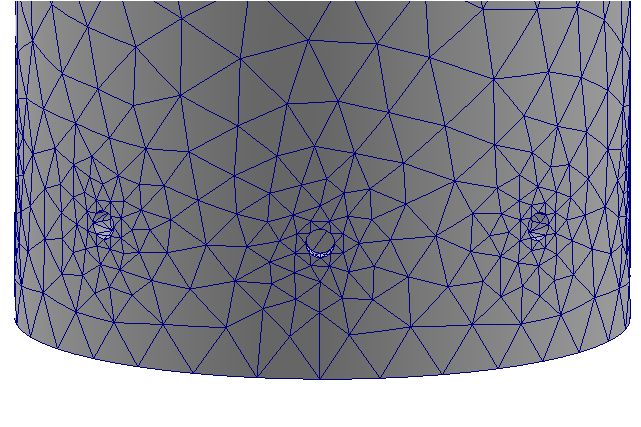
\includegraphics[width=\textwidth]{../report_assets/fine_mesh.png}
        \caption*{Mesh with Fine Setting}
    \end{minipage}
    \hfill
    \begin{minipage}{0.45\textwidth}
        \centering
        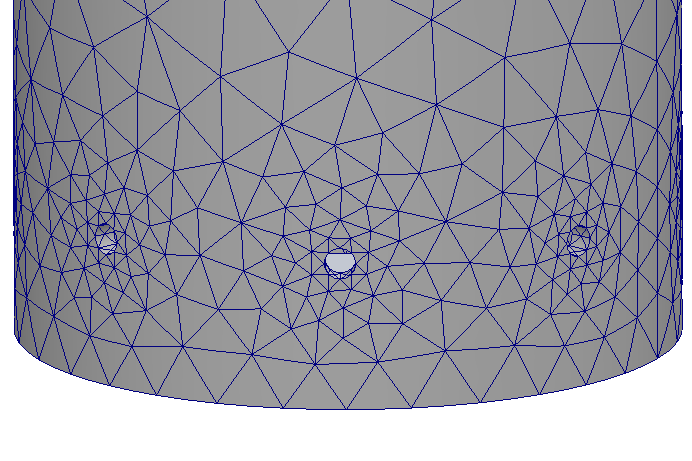
\includegraphics[width=\textwidth]{../report_assets/medium_mesh.png}
        \caption*{Mesh with Medium Setting}
    \end{minipage}
    \caption{Solidworks Meshes Used}\label{fig:solidworks-fea}
\end{figure}
The force on the bolt holes was assumed to be the force on the end cap face from a 7 bar pressure differential, ignoring any affect from the o-ring. A force of 3,010N was found through the equations below.
\[
F = P \cdot A
\]
\[
3,010N = 700,000Pa \cdot (0.037mm^2 \cdot \pi)
\]
This force was then applied to only the bottom half of the hole cross-section as this is where the bolt would contact the surface. The acrylic was modelled as 

To investigate the hoop stress rupture failure method, hand calculations were conducted.
Upon construction of the tank, it was hydrostatically pressure tested to a pressure of 8 bar. At the time of testing, it was known that the safety factor of the design was lower than standard and therefore was not pressurised above the 8 bar limit for fear of damaging the tank. This was definitely not ideal but given the time and budget constraints, manufacturing a new powder hopper was not an option.

\section{Piston Design}\label{sec:piston}
The piston's main function in this design is to constrain the powder to the outlet of the device. By modelling the sand as a fluid, the force required by the piston to pack the sand against the outlet can be calculated through the hydrostatic pressure equation, seen below. 
\[
P = \rho * h * g
\]
This pressure has to balance the pressure differential across the piston from the flow and the additional frictional force on the tank walls to ensure the powder is packed at the outlet. Due to the non-linear nature of granular material's affect on friction, modelling this prior was deemed outside of the scope of the project. Additionally, manufacturing imperfections in both the tank tube and piston prevent a detailed study of the flow around the piston so the expected pressure differential was also too complex to model. While the piston design has the greatest potential for optimising the system, time constraints of the project prevented further analysis.

Because of these complexities, the first design, seen in \autoref{fig:piston_geom} (a), was modelled after a previous study that found a gear-like geometry to have the best performance in the gas-permeable powder feed system tested~\cite{TANG2023118406}. 
\begin{figure}[htbp]
    \centering
    
    \begin{minipage}{0.3\textwidth}
        \centering
        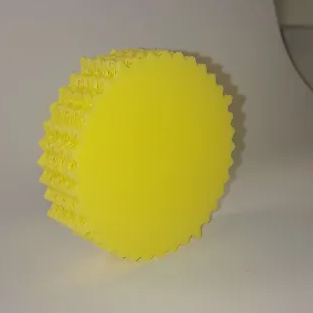
\includegraphics[width=\textwidth]{../report_assets/piston_1.png}
        \caption*{(a) First Design}\label{fig:piston_geom_1}
    \end{minipage}
    \hfill
    \begin{minipage}{0.3\textwidth}
        \centering
        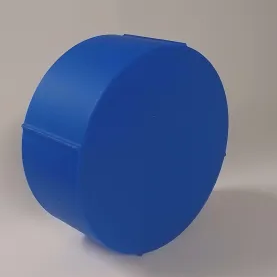
\includegraphics[width=\textwidth]{../report_assets/piston_2.png}
        \caption*{(b) Second Design}\label{fig:piston_geom_2}
    \end{minipage}
    \hfill
    \begin{minipage}{0.3\textwidth}
        \centering
        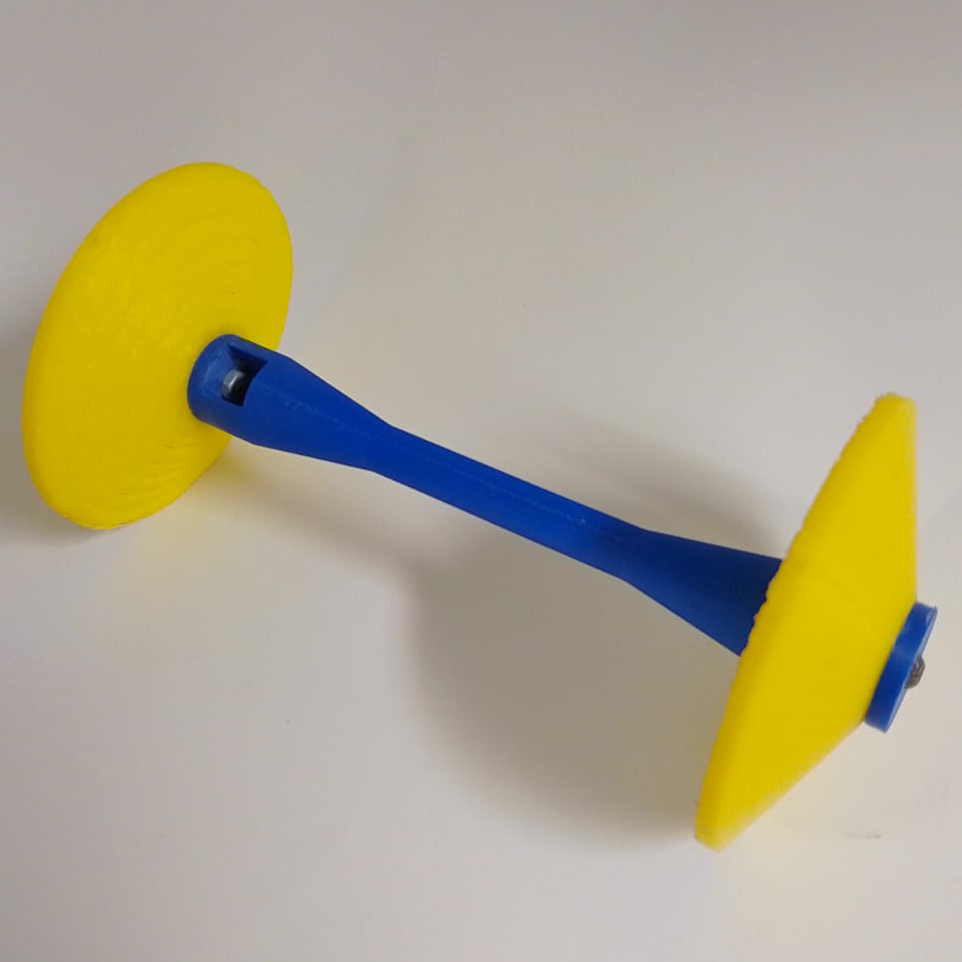
\includegraphics[width=\textwidth]{../report_assets/piston_final.png}
        \caption*{(c) Final Design}\label{fig:piston_geom_3}
    \end{minipage}
    \caption{Piston Design Iterations}\label{fig:piston_geom}
\end{figure}
This was designed under the assumption that the high pressure within the tank would not equalise with the pressure inside the print quickly enough, causing it to crumple or deform. Therefore when 3D printing the model, the wall layers were not printed to allow for this equalisation. In preliminary testing, this design did not generate enough pressure force to be moved down the tank, motivating the need for another iteration.

Building off this insight, the second piston was designed to try and constrict the flow around the piston as much as possible to generate a higher pressure force. As discussed in \autoref{sec:first-test}, this piston did move from the pressure but immediately became jammed by the sand, motivating the next redesign focused on preventing this jamming.

The final piston consists of 2 3D printed TPU cones, 3mm thick, and a connecting rod made of PLA. The flexibility of the TPU provided much needed resiliance against jamming as individual grains could be flexed around or over to continue compacting the rest of the sand. Along with the material change, longer pistons are more resiliant to jamming through axis-misalignment so the connecting rod was designed to be 100mm to incorporate this. Not only does the 2 plates and rod configuration allow for the piston to be lighter weight than a fully TPU piston, it also allowed each face to be thinner and therefore give less contact area for friction or powder jamming. Furthermore, the flexibility of the TPU allowed for the piston face to fully cover the cross section of the tank. This is because the manufacturing imperfections like varying cylindricity or diameter down the tank have less of an impact on the friction experienced by the piston. Consequently, allowing for a higher pressure differential and, in turn, more consistent compaction of the sand against the outlet.
% why is axis-misalignment solved by making it longer

\section{Expected Behaviour}
To predict the behaviour of the design, parallels were drawn from research looking at fluidising powder feed systems for metal powder engines. It has been proposed that you can split the analysis of the flow behavior within the tank of these systems into two regions: a dense phase moving area before the cone and a fluidising region afterwards~\cite{Tang22}. This has been interpreted to produce the behaviour seen in \autoref{fig:expected}. 
\begin{figure}[htbp]
    \centering
    
    \begin{minipage}{0.6\textwidth}
        \centering
        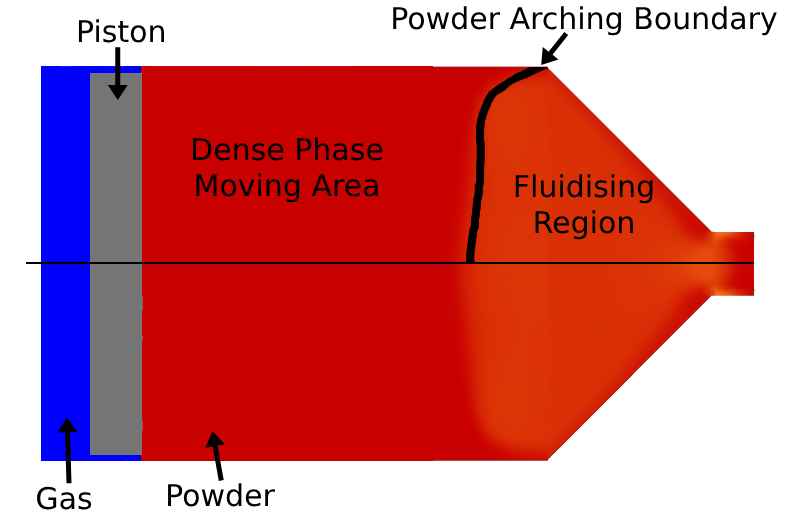
\includegraphics[width=\textwidth]{../report_assets/expected_result.png}
        \caption{Expected Behaviour}\label{fig:expected}
    \end{minipage}
    
\end{figure}
This analysis assumes arching occurs, previously discussed in \autoref{sec:bulk-powder}, due to the presence of the tube cone interface and pressure from the piston, constraining the powder into the arched structure. The proposition is also supported by two findings from literature. The first being that the velocity of the piston has a linear relationship with the mass flow dispensed from the system~\cite{SUN201630}. The second is that the force on the piston initially provides a positive correlation with mass flow rate but then saturates and an increase in force on the piston no longer produces any increase in mass flow rate~\cite{LI2021712}. 

If, in a system where the piston provides little force on the powder, the fluidising region undergoes expansion, analogous to bed expansion, passed the cone-tube interface (leftwards on the diagram). Then, applying more force to the piston would compress this region down, meaning a higher density of powder in the fluidising region, therefore more particles to be entrained out so a higher mass flow rate. In the case the force on the piston is greatly increased, the fluidising region would be compressed down into the cone and the dense phase moving area would reach the cone-tube interface. This would allow arching to occur and the additional force would be transferred through the powder into the cone, no longer compressing the fluidising region. In this case the behaviour seen in research would occur, where at a certain force, additional pressure on the piston produces no additional mass flow rate. 

This explaination of the system puts very high demand on the design of the piston as it controls both the force on the powder and the flow rate of fluidising gas. These two quantities are functions of the inlet pressure and the fact they are coupled in a non-trivial way is not condusive of an easily controllabile design but comes with considerable benefits in terms of miniaturisation, a compromise deemed satisfactory.

\section{Experimental Setup}
The experimental set up was designed to verify the expected behaviour of the fluidising powder feed system under terrestrial conditions to better estimate it's behaviour under microgravity. The core aims were to record the consistency of the powder mass flow rate, verify that changing the pressure upstream of the tank leads to a change in mass flow rate and document any behaviours the system may exhibit that would impact it's suitability for space applications.

\subsection{Layout}
The default layout, seen in \autoref{fig:experimental-setup}, was used to perform most of the testing, with modifications outlined in the sections where they occur. 
\begin{figure}[htbp]
    \centering

    \begin{minipage}{0.6\textwidth}
        \centering
        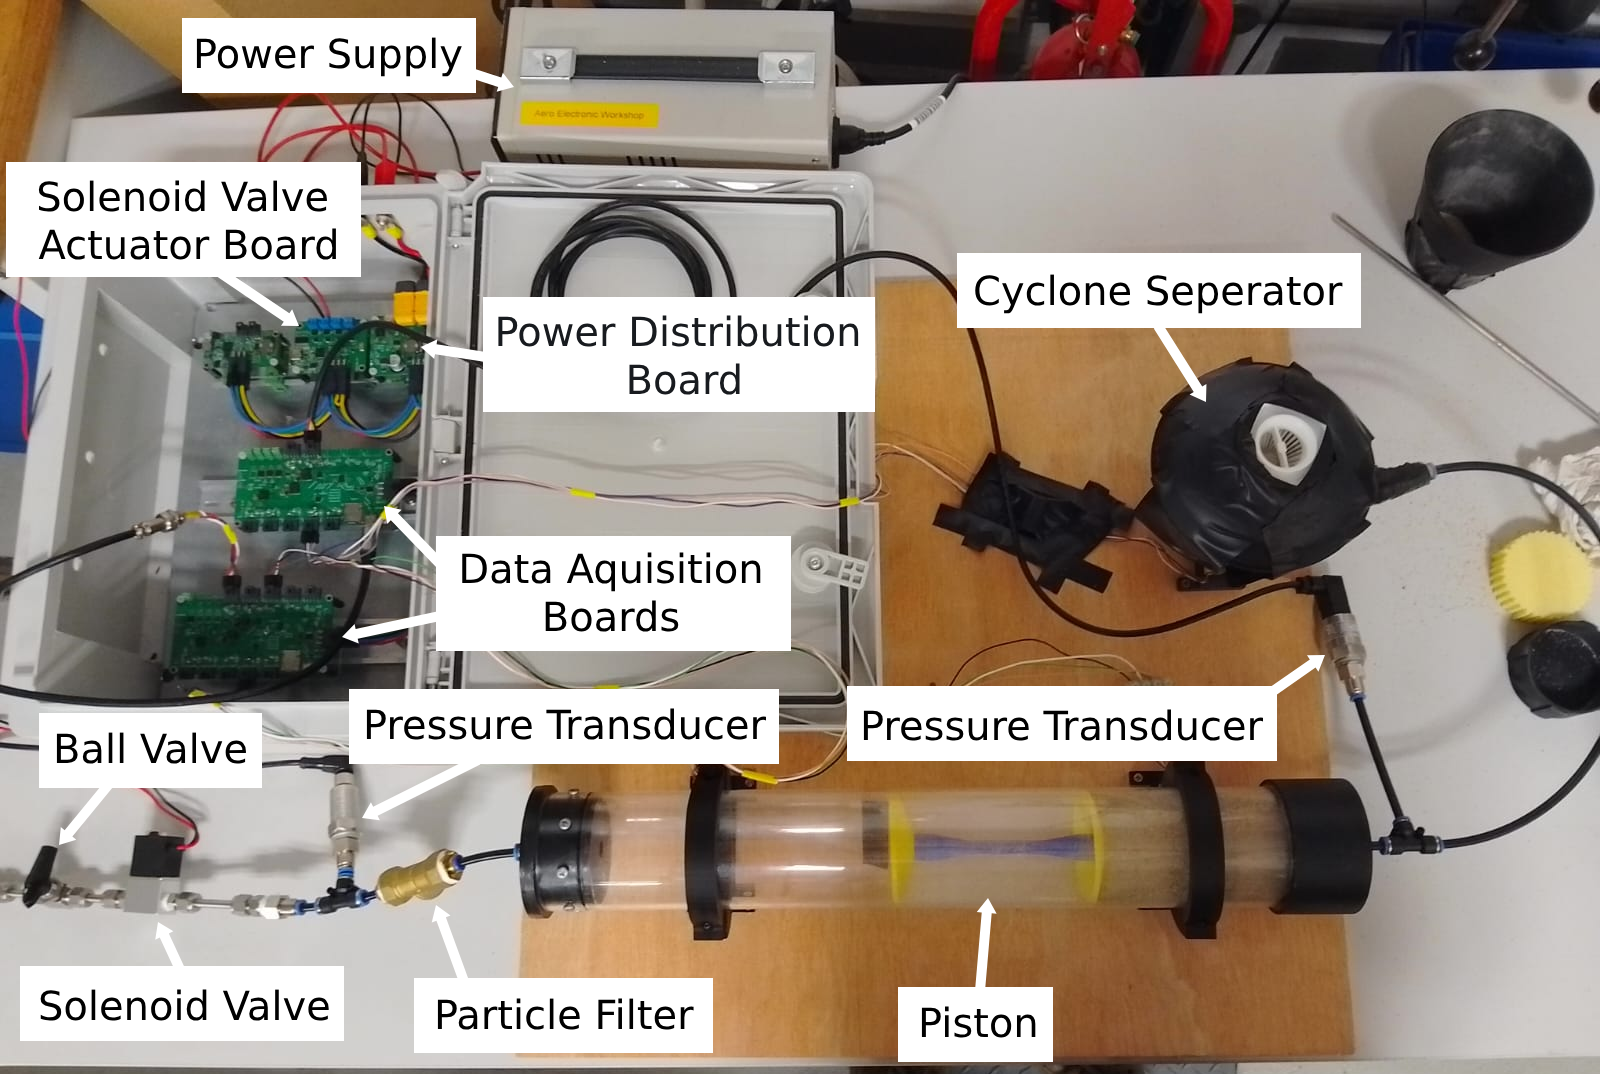
\includegraphics[width=\textwidth]{../report_assets/setup_annotated.png}
        \caption*{Annotated Image of Setup}
    \end{minipage}
    \hfill
    \begin{minipage}{0.3\textwidth}
        \centering
        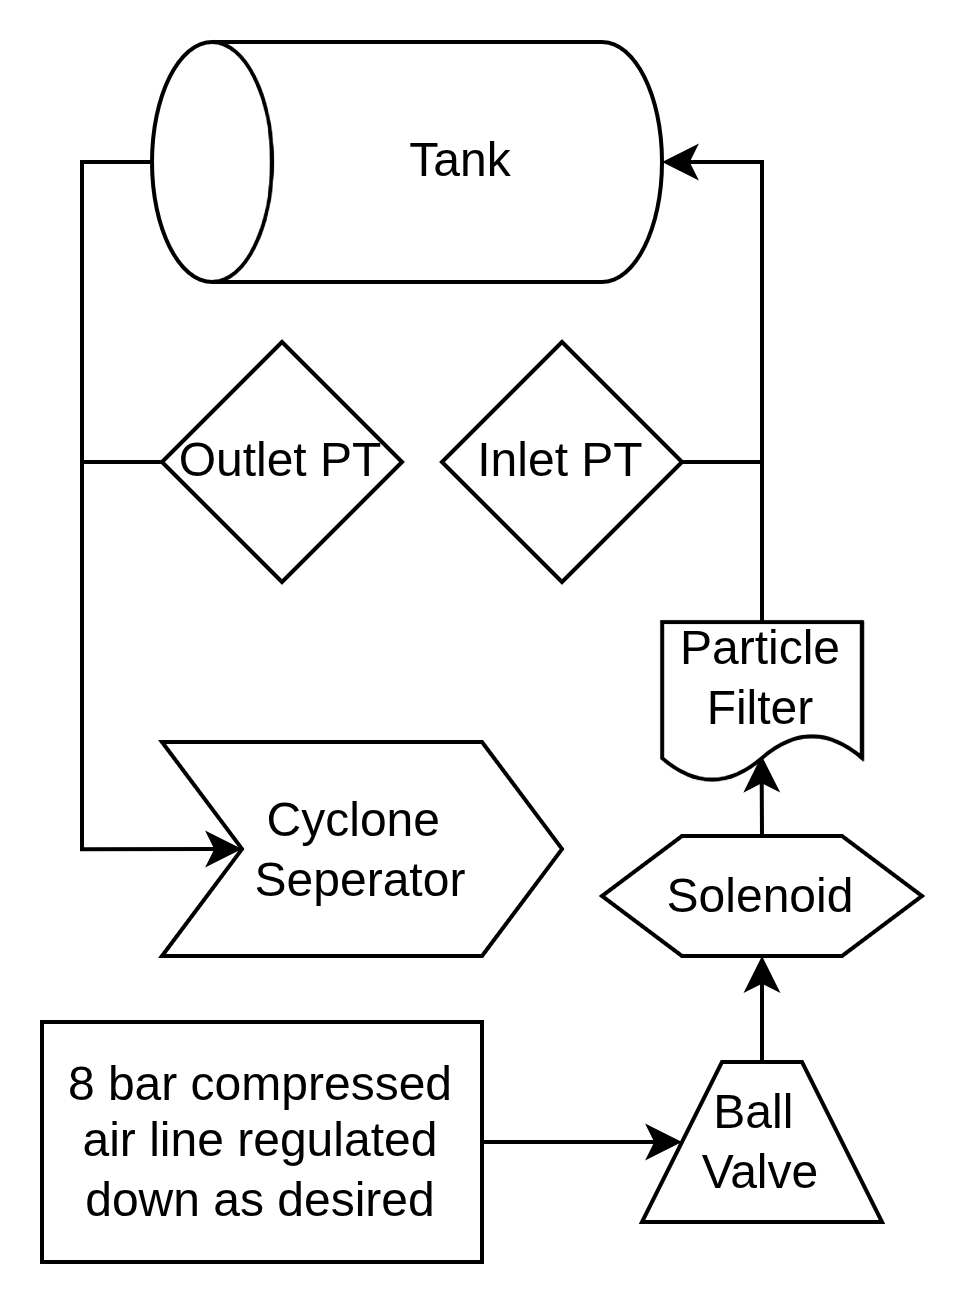
\includegraphics[width=\textwidth]{../report_assets/drawio_setup_vertical.png}
        \caption*{Systems Diagram of Setup}
    \end{minipage}
    \caption{Experimental Setup}\label{fig:experimental-setup}
\end{figure}
The testing was undertaken inside Imperial College's Hypersonic Lab which maintains no climate control. It was assumed that the system would not behave noticeably differently under the slightly varying teperatures and pressures that occured over the testing.

\subsection{Data Acquisition and System Actuation}
To capture the system's behaviour, a combination of video recordings, load cell readings and pressure transducer readings were taken during each test. The placement of the sensors is shown in \autoref{fig:sensors} and their values were read with the use of custom electronics designed by the Imperial College London Rocketry team.
\begin{figure}[htbp]
    \centering

    \begin{minipage}{0.45\textwidth}
        \centering
        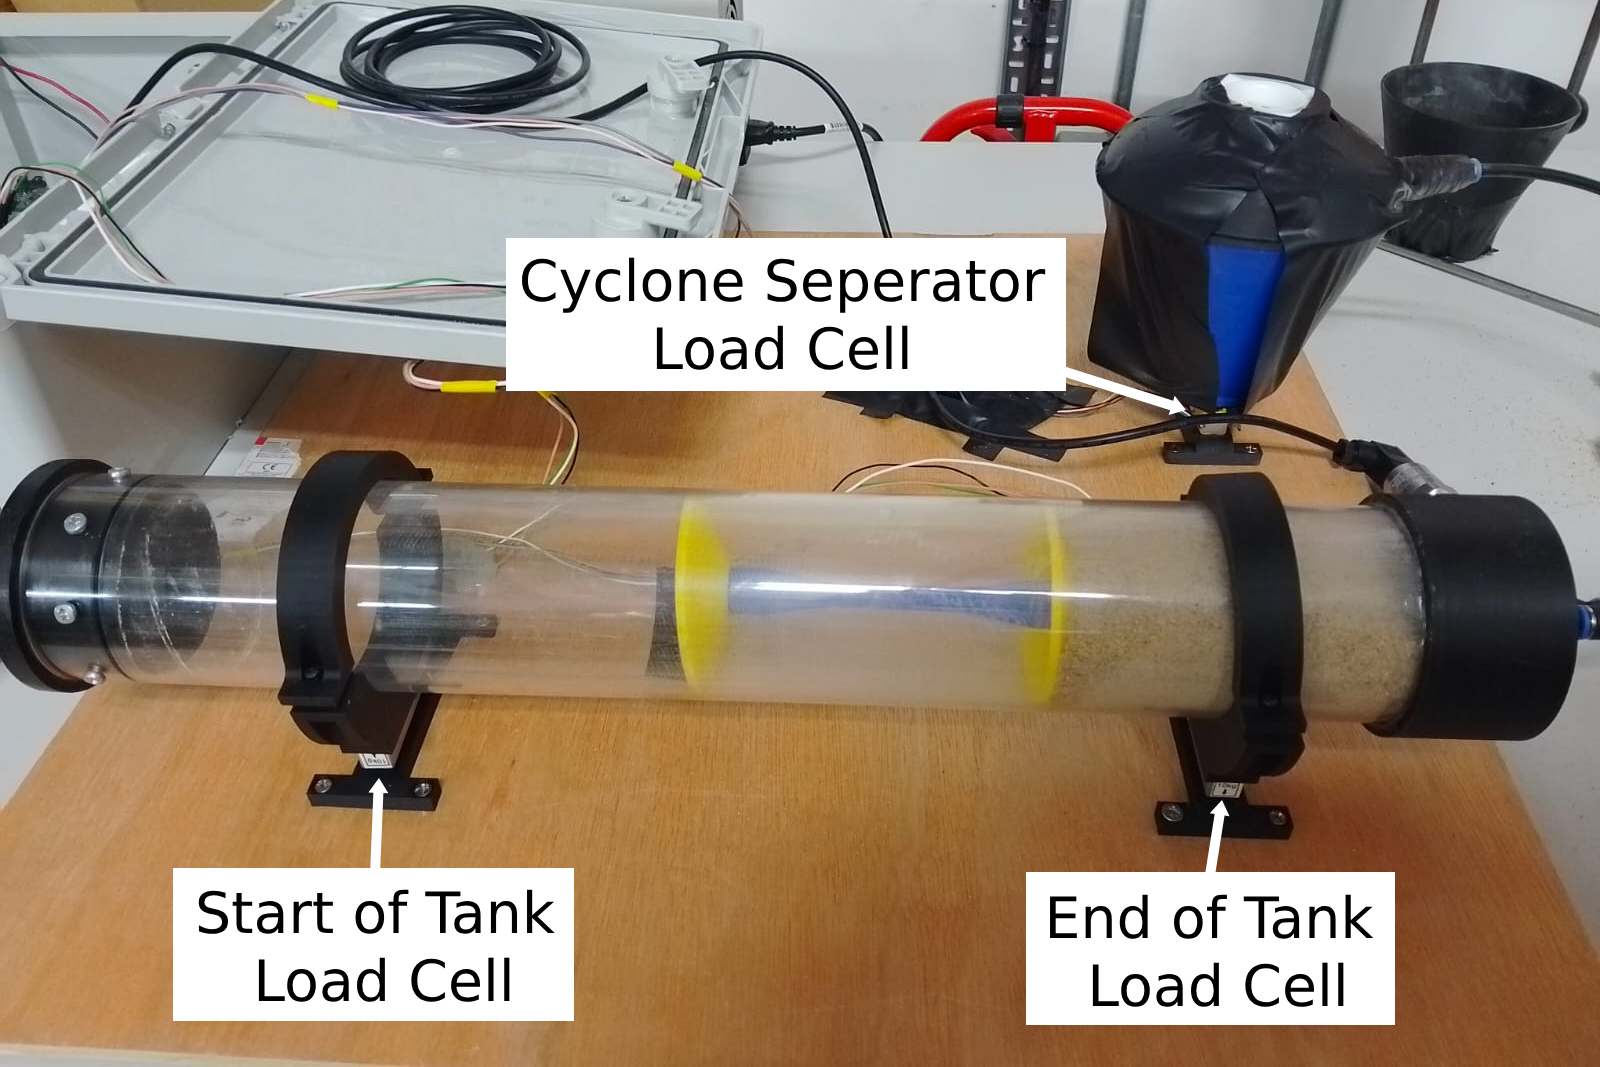
\includegraphics[width=\textwidth]{../report_assets/load_cell_configuration.png}
        \caption*{Load Cell Placement}
    \end{minipage}
    \hfill
    \begin{minipage}{0.45\textwidth}
        \centering
        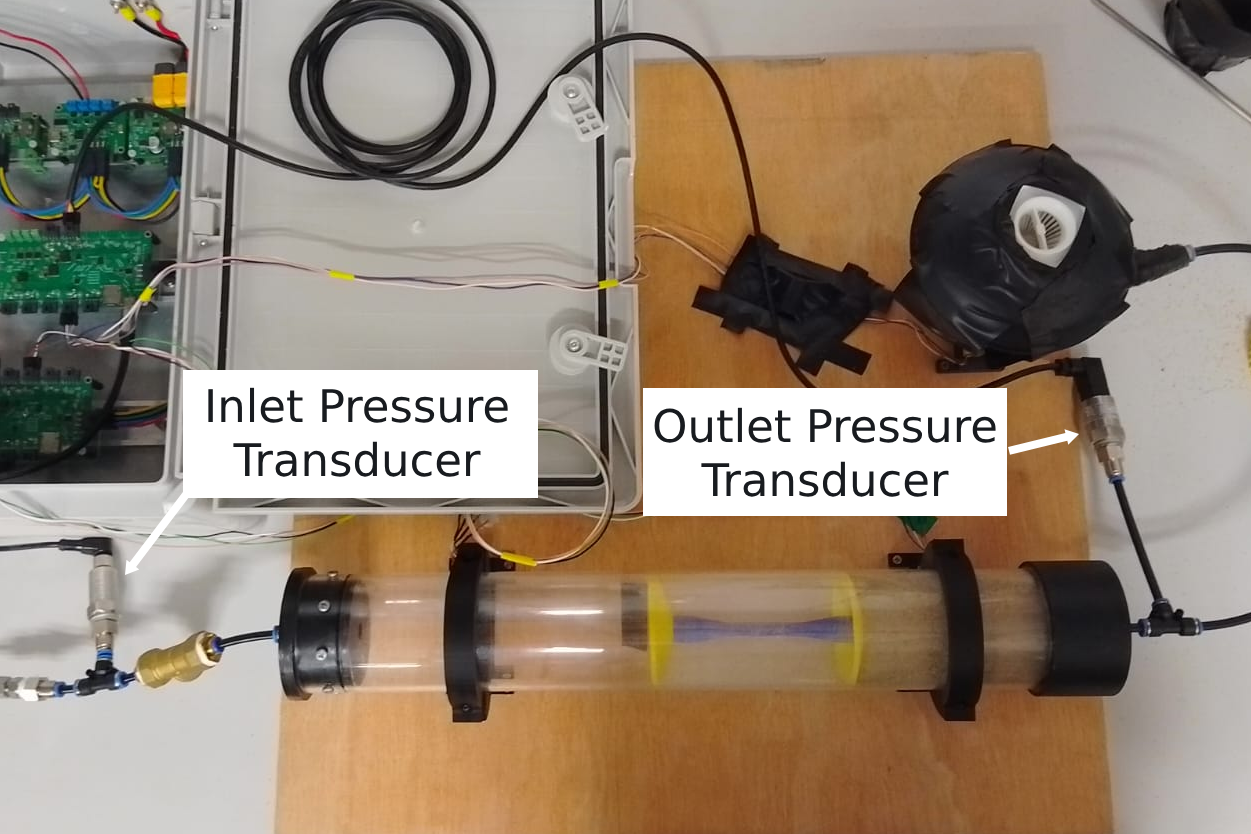
\includegraphics[width=\textwidth]{../report_assets/pressure_transducer_configuration.png}
        \caption*{Pressure Transducer Placement}
    \end{minipage}
    \caption{Sensor Placement in Experimental Setup}\label{fig:sensors}
\end{figure}

A computer was connected to the boards and data was logged to it as well as being presented on a bespoke user interface, shown in \autoref{fig:grafana}. The solenoid could also be opened and closed through the dashbaord, allowing for safe operations as all the information and control was in one place.
\begin{figure}[htbp]
    \centering

    \begin{minipage}{0.95\textwidth}
        \centering
        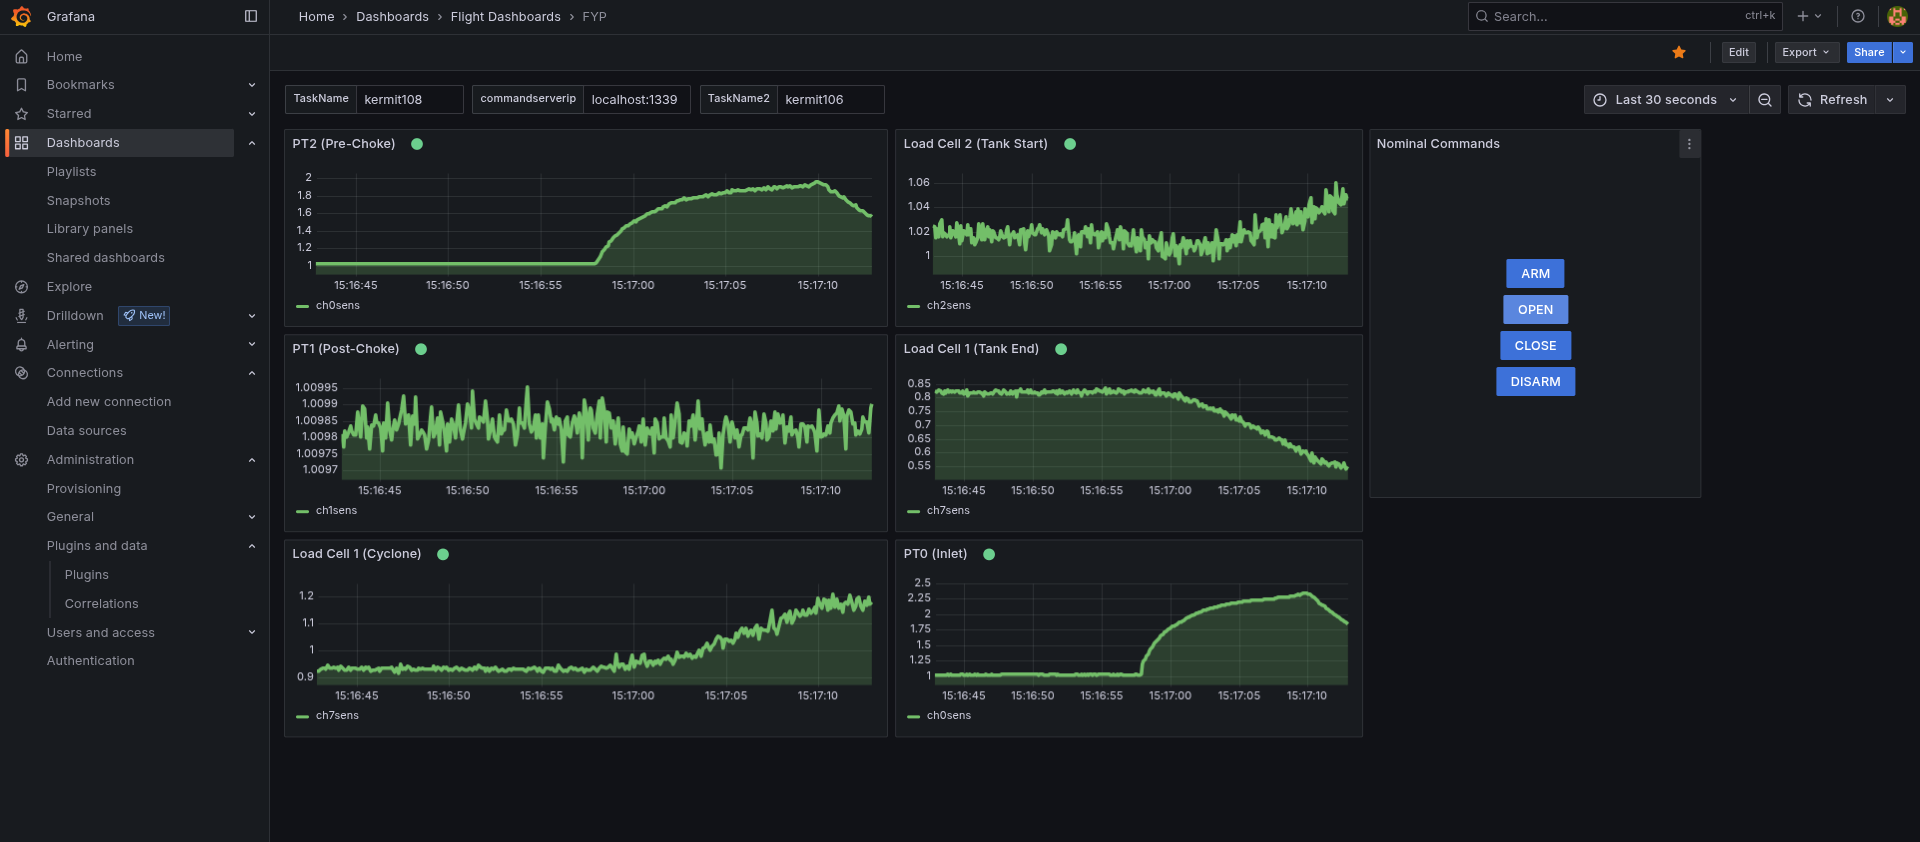
\includegraphics[width=\textwidth]{../report_assets/grafana.png}
        \caption{Testing Dashbaord}\label{fig:grafana}
    \end{minipage}

\end{figure}
Due to budget constraints only cheap pressure transducers and load cells were used. Given this, perfect calibration of the sensors was not as much of a priority. To calibrate the load cells, the data aquisition baord was configured to record the raw values out put by the analog to digital converter (ADC) at both the unloaded, 0kg, state and then with a mass, measured at 0.746kg, placed on it. Since the load cells are a linear sensor, these two points give a gradient and y-intercept to map the ADC counts to. The same procedure was done to calibrate the pressure transducers except using a mechanical pressure gauge and the compressed air line to record 1bar and 4bar ADC outputs.

An older setup of the experiment included a choke point just after the outlet of the tank. This was because previous literature proposed that fluidising systems where one part of the gas-solid flow is in choking conditions had been found to be simpler to control~\cite{SUN201630}. Due to the grain size of the sand, this chokepoint got clogged in testing so was removed. As there was a pressure transducer before and after the chokepoint, this explains the naming scheme in \autoref{fig:grafana} and why the pre-choke pressure data is just noise as it was no longer connected.

\subsection{Cyclone Seperator and Measurement Method}
The two most common methods of measuring mass flow rate for this kind of system are using a displacement transducer to measure how far down the tank the piston is or measuring the mass of the powder after it has been fed out of the tank~\cite{SUN201630}\cite{LI2021712}\cite{Tang22}.
 The displacement transducer method indirectly measures the mass flow by using the near incompressibility of the powder and the assumption of a constant packing density to form a linear relationship between the movement of the piston and the volume of powder dispensed~\cite{SUN201630}. The direct method requires some method of seperating the gas and powder and then measures the powder. 

WHY dID I CHOSE THE SEPERATOR INSTEAD OF THE Displacement
EDITS TO TANK UNIDEAL GIVEN PRESSURE RATING things
NEED TO CAPUTRE AIR ANYWAY FOR HEALTH AND SAFETY SO EASIER TO implement
MAYBE CITE COMPARISON PAPER

To seperate the gas and powder, a cyclone seperator was used, seen in \autoref{fig:cyclone}.
\begin{figure}[htbp]
    \centering

    \begin{minipage}{0.3\textwidth}
        \centering
        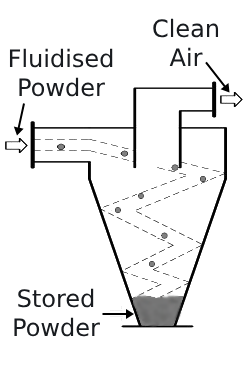
\includegraphics[width=\textwidth]{../report_assets/cyclone_diagram.png}
        \caption*{(a) Cyclone Seperator Diagram}
    \end{minipage}
    \hfill
    \begin{minipage}{0.3\textwidth}
        \centering
        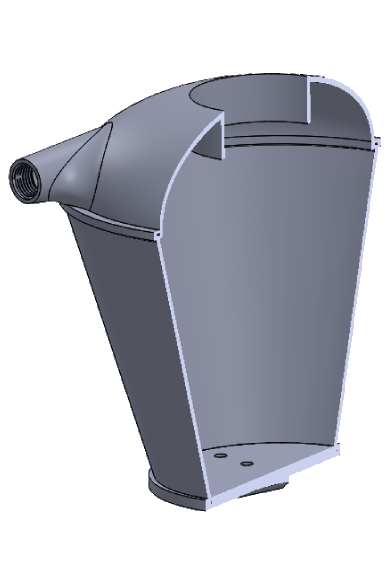
\includegraphics[width=\textwidth]{../report_assets/cyclone_cad.png}
        \caption*{(b) CAD Model of Seperator}
    \end{minipage}
    \hfill
    \begin{minipage}{0.3\textwidth}
        \centering
        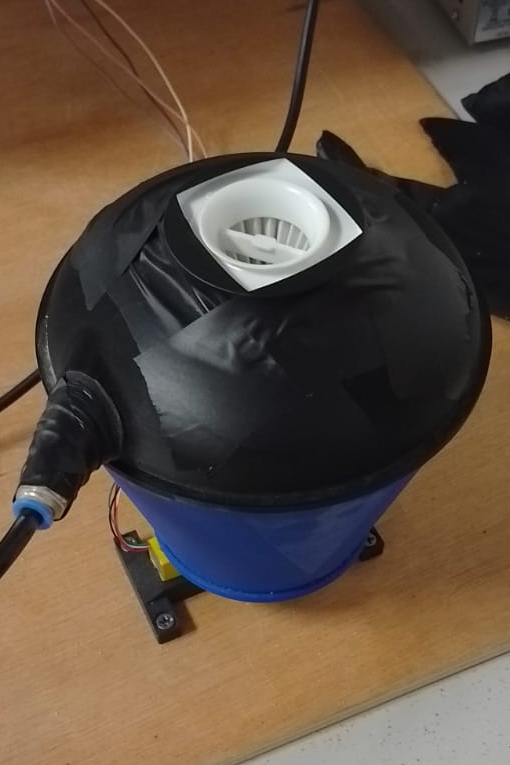
\includegraphics[width=\textwidth]{../report_assets/cyclone_done.png}
        \caption*{(c) Cyclone Seperator}
    \end{minipage}
    \caption{Sensor Placement in Experimental Setup}\label{fig:cyclone}
\end{figure}
A cyclone separator works by using centrifugal force to separate the sand from the air. As the mixture enters the cyclone chamber tangentially at high speed, it spins rapidly, causing the denser particles to move outward and fall to the bottom, while the cleaner air exits through the top center. As shown in \autoref{fig:cyclone} (c), a dust filter used in vacuum cleaners was used to ensure any fine grains, not captured by the seperator, do not make it out into the air. This was attached to the 3D printed model using PTFE tape and a friction fit, then taped down for added support. The seperator was printed in 3 parts, the top that can be removed to empty out the sand, the walls and the base with screw holes to mount to the load cell.
% The direct cyclone seperator method was chosen to record mass flow, with a back up recording of the mass of the tank during operations. This is because the sand needs to be contained after exiting the tank as inhalation of silica particles can lead to long term health conditions. Therefore, the direct method was chosen as

\subsection{Powder}
While typical powders used in CSAM are $5\,\mu\mathrm{m}$ to $100\,\mu\mathrm{m}$~\cite{Vaz2023}, budget constraints resulted in sand being the optimal granular material safe enough to work with. This will definitely affect the behaviour of the system but to what extent is unknown. A rudimentary attempt was made to measure the particle diameter using a micrometer but given the time limitations, no formal attempt was made to characterise the diameter distributions or average diameter. As mentioned in \autoref{sec:numerical-setup}, the bulk density, that being the density of the sand including the volume occupied by air, was measured by recording the mass of the sand in a bowl and then filling the same bowl with water.

% For safety and due to the limited budget, sand was used as the powder. This is one of the greatest areas for improvement, i dont actually know what size the powder is or the distribution of those sizes. This powder has been measured to have [density = 1.4g/cm3]

% \newpage

\subsection{Procedure to Characterise Pressure Source}\label{sec:pressure-source-procedure}
Due to safety and ease of handling, the pressurised air supplied into the system came from a compressed air line. As mentioned in \autoref{sec:first-test}, the pressure readings from preliminary testing were lower than expected so an attempt at characterising the air supply was made. 

To do this, the steady-state flow through system without any piston or sand was investigated by measuring the static pressure before and after the tank at different regulator settings. Tuning of the regulator was consistent across all experiments conducted and was done as follows. The system was closed by replacing the inlet pipe into the tank with a pushfit end cap, as seen in figure \autoref{fig:systems-diagram-end-cap}.
\begin{figure}[htbp]
    \centering
    \begin{minipage}{0.60\textwidth}
        \centering
        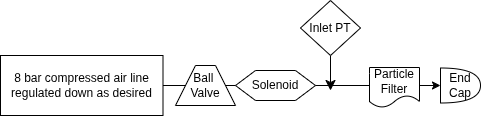
\includegraphics[width=\textwidth]{../report_assets/end_cap.drawio.png}
        \caption{System Diagram of Closed System}\label{fig:systems-diagram-end-cap}
    \end{minipage}
\end{figure}
The regulator integrated into the compressed air line was then adjusted using the inlet pressure transducer readings as a reference. While there was a gauge on the regulator, it was consistently reading 0.2 to 0.3 bar higher than the pressure transducers in the system or manual pressure gauges used so was deemed unreliable. Once the pressure was tuned on the regulator, the valves were closed, the end cap was removed and the tube was reattached to the tank, returning to the default configuration. 

Confirmation of the lower than expected static pressure readings motivated follow up tests to eliminate possible sources of human error in the system setup. The pressure regulator integrated into the compressed air line was checked first by including another gauge closer to the system and fully opening the integrated one. If the static pressure losses were because of the 2 meters of nylon tube from the air line to the experimental setup, this would also have been highlighted.

Additionally, the solenoid valve could have had a very small orifice area, chocking the flow just before the pressure transducer and explaining the loss in static pressure so this was also investigated by removing the component and running additional tests.

\subsection{Procedure to Characterise Full System}
To compare the system behaviour at each pressure inlet, 

The tank was fist prepared by removing the inlet end cap and placing in the piston. This was positioned at the start of the tank to lower the chance that the piston gets stuck on the sand that forms a ramp, seen in \autoref{fig:sand-ramp}.
\begin{figure}[htbp]
    \centering
    
    \begin{minipage}{0.45\textwidth}
        \centering
        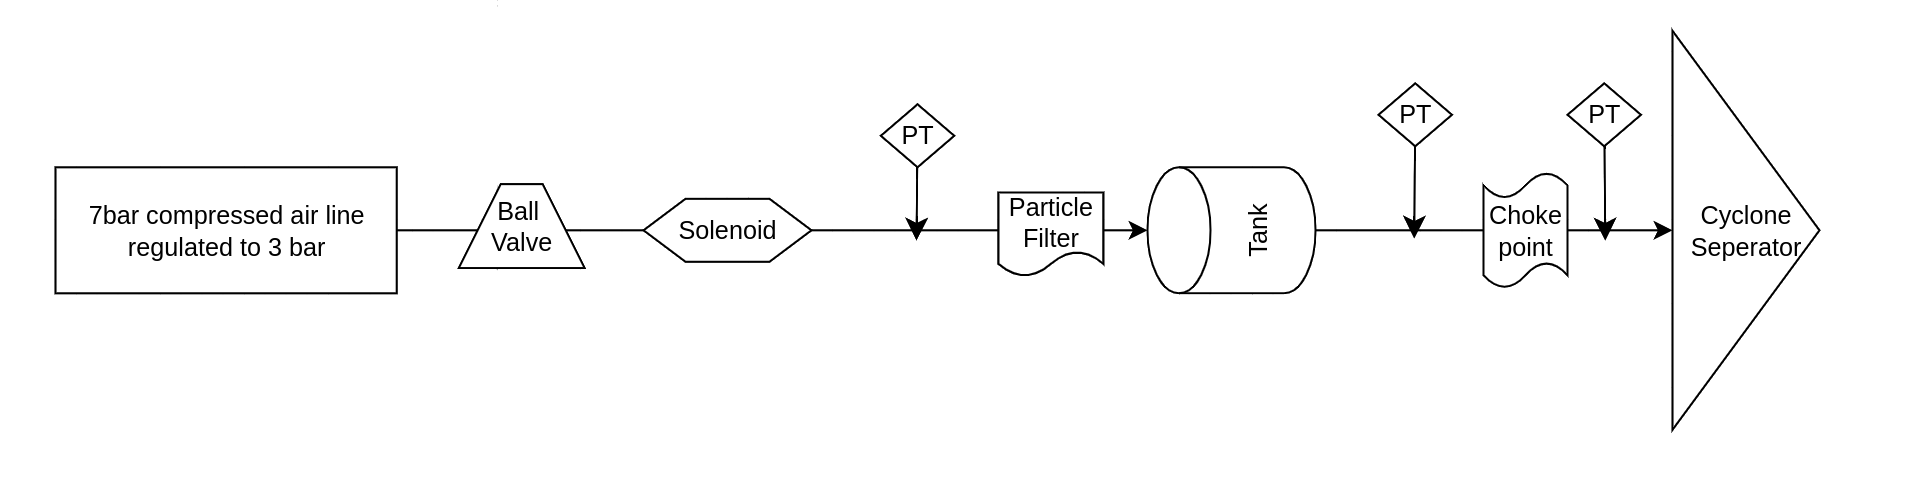
\includegraphics[width=\textwidth]{../report_assets/systems_diagram.png}
        \caption{Systems diagram.}\label{fig:sand-ramp}
    \end{minipage}
    \hfill
    \begin{minipage}{0.45\textwidth}
        \centering
        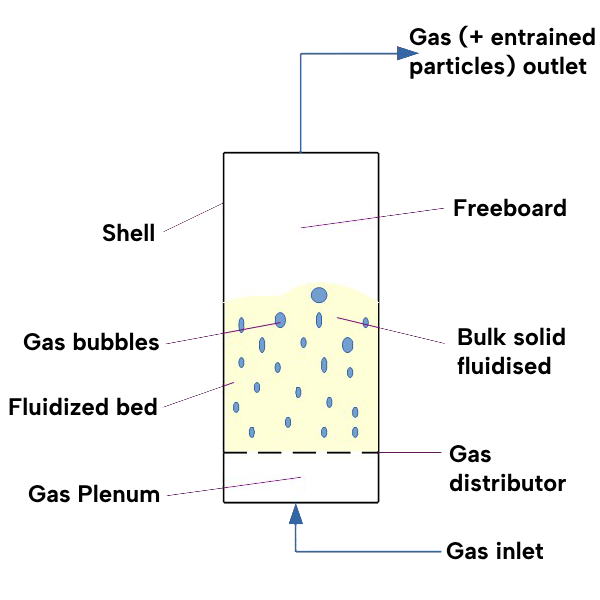
\includegraphics[width=\textwidth]{../report_assets/Fluidised_Bed_polished.png}
        \caption{Pic of experiment.}\label{fig:wawaweewa}
    \end{minipage}
    
\end{figure}
If the piston has time to accelerate from far away, then it was found to be more likely to sweep that ramp sand forwards with its movement and fully pack the sand into the outlet instead of getting stuck. Next the female pushfit fitting was removed from the outlet of the tank and 1000-1020g of sand was measured out and put into the tank through the use of a funnel. Once the sand had filled the tank, the pushfit fitting was reattached and a tube with an end cap was placed over the outlet. The tank was then rotated such that the outlet was facing down and tapped to ensure no sand was stuck to the walls close to the piston, preventing successful startup. Then the tank was placed on the load cell stands, ensuring that the system starts with sand fully covering the cross section of the tank close to the outlet. Once placed down, the end cap tube was removed and the tube leading to the cyclone seperator was connected. The cyclone seperator was then taped down to reduce the likelyhood the lid pops off. It is thought that this was only necessary due to the undersizing of the cyclone seperator but a 3rd iteration on that was deemed unnecessary. Once the system was set up, the pressure regulator was tuned like in \autoref{sec:pressure-source-procedure}, closing the system then 
\newpage
\section{Numerical Setup}\label{sec:numerical-setup}
\subsection{Numerical Setup to Characterise Pressure Source}
To provide an additional angle into the investigation of source pressure behaviour, seen in \autoref{sec:static_test}, an axisymmetric simulation was conducted of the system without a piston or powder in the tank. The geometry used can be seen in \autoref{fig:geometry_static_sim}, noting the two vertices in the geometry outlined to record the numerical values of pressure at locations similar to the pressure transducers in the experimental setup.
\begin{figure}[htbp]
    \centering
    
    \begin{minipage}{0.9\textwidth}
        \centering
        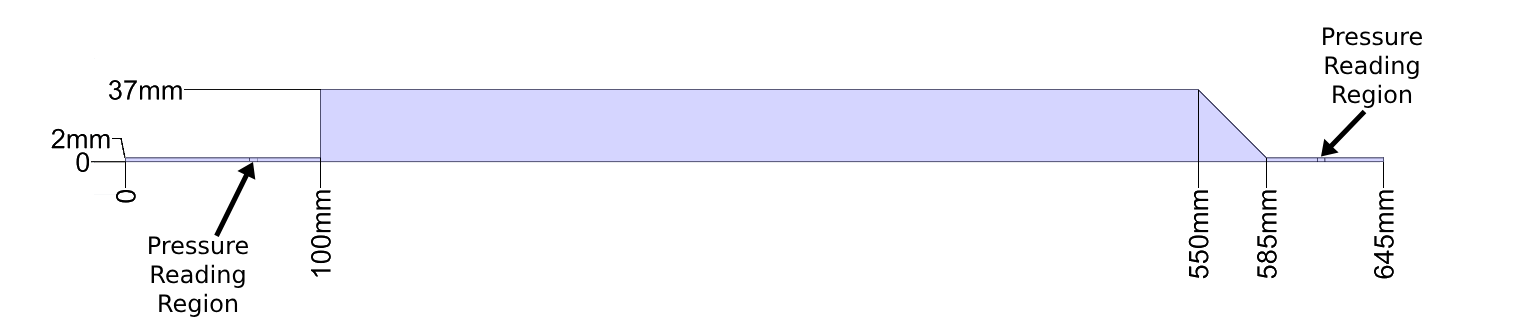
\includegraphics[width=\textwidth]{../report_assets/geom_pressure_losses.png}
        \caption{Geometry of Simulation to Characterise Pressure Source}\label{fig:geometry_static_sim}
    \end{minipage}
    
\end{figure}
An axisymmetric model was chosen as it requires far fewer computations due to the lower number of cells, while still preserving the pressure quantities of the 3D physics. This was possible as it is expected that there would be no angular dependence around the axis of revoluiton and no swirling is expected to occur. Because of the reduced time requirement of the axisymmetric model, the mesh used 0.1mm square cells to produce a high resolution analysis of the flow. The inlet was modelled as a pressure inlet with a stagnation pressure of 2 bar and the outlet was a pressure outlet at atmospheric conditions. The gas used was air under standard operating conditions as this assumed to be close to what is output from the compressed air line.
\subsection{Numerical Setup to Characterise Full System}
To investigate how well the design would translate to the space environment, numerical simulations to observe key flow features were conducted. Given that there is no experimental data on fluidisation under microgravity present in literature, options to verify the validity of the simulations are limited. Therefore, attempts to show well documented behaviours like the relationship between piston velocity and mass flow rate were made. Anchoring the validitiy in these relationships given no other options. The scope of the project reduced the simulation methods to pre-existing software and Ansys Fluent was chosen as it could perform moving mesh simulations as well as two phase flow simulations with limited prerequisit knowledge.

Given the complexity of the simulation, an extensive testing campaign was undertaken with only the final simulation outlined below. The simulation software chosen has a limit on the number of cells a mesh can have when using the student license. This restricted the modelling options to axisymmetric and 2D. Given that gravity is not an axisymmetric phenomenon and the tank was oriented horizontally in experiments to limit the affect of gravity on the system, a 2D simulation was conducted. 

Experimentation with the mesh found that 1mm squares was optimal with respect to simulation stability and run time. A time step of 0.0001s was used meaning only timeframes were analysed but this 
\begin{figure}[htbp]
    \centering

    \begin{minipage}{0.45\textwidth}
        \centering
        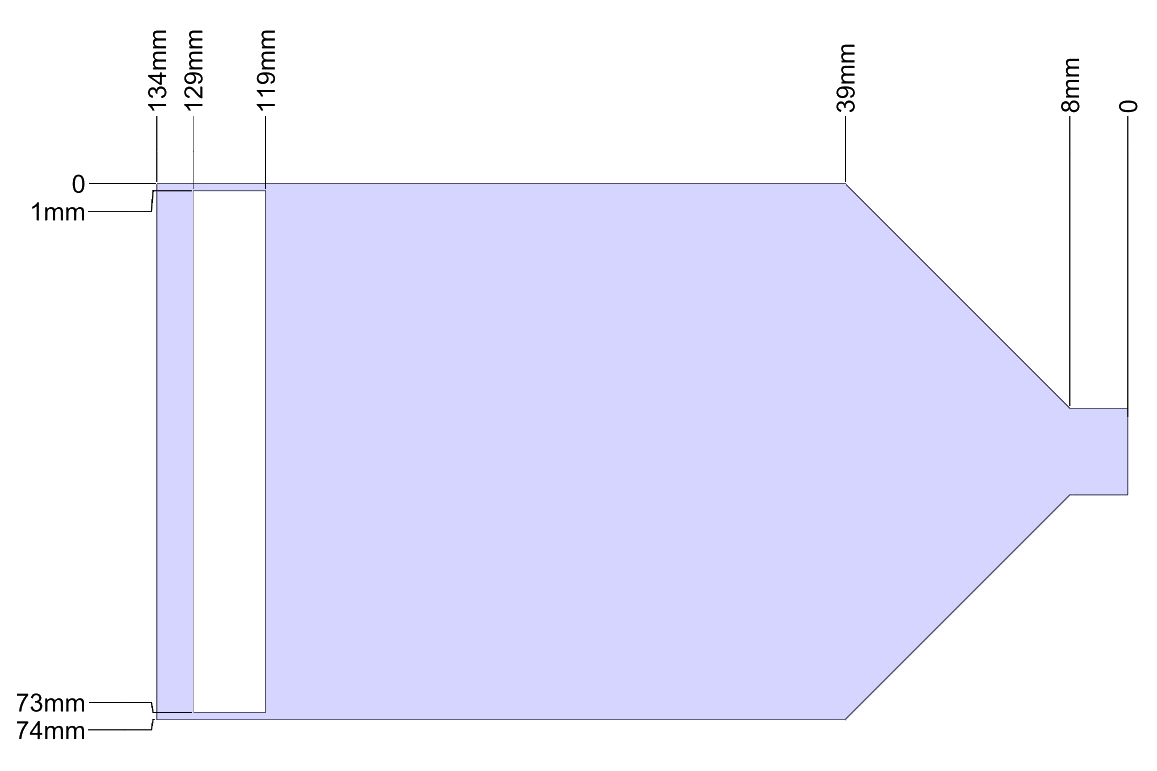
\includegraphics[width=\textwidth]{../report_assets/big_sim_geom.png}
        \caption{2D Geometry of Tank}\label{fig:2D-tank}
    \end{minipage}
    \hfill
    \begin{minipage}{0.45\textwidth}
        \centering
        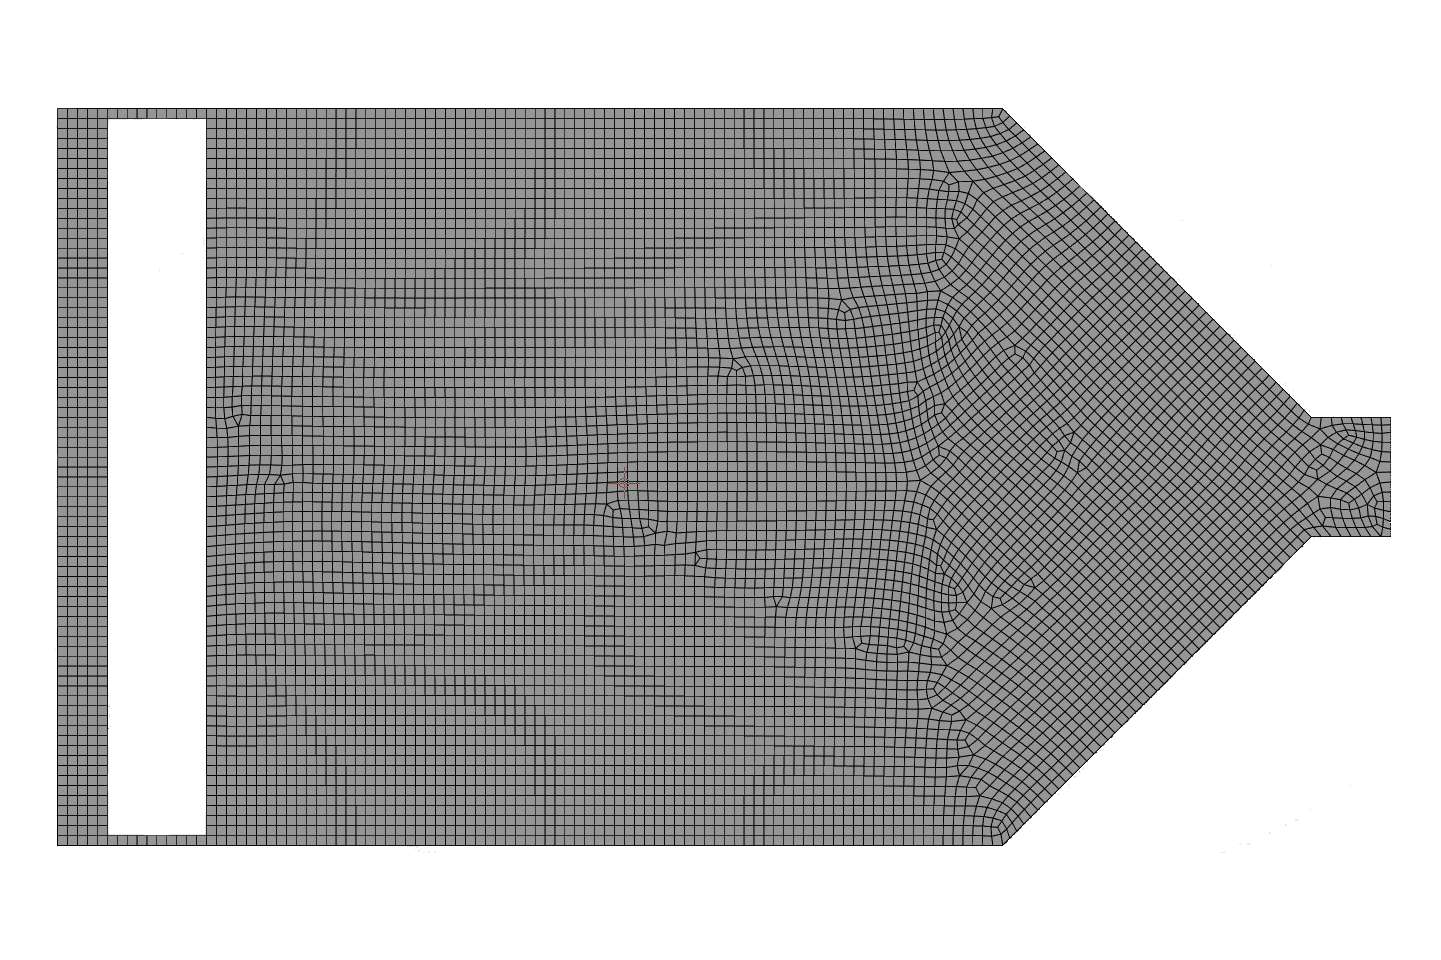
\includegraphics[width=\textwidth]{../report_assets/big_sim_mesh.png}
        \caption{Mesh of Tank}\label{fig:mesh-tank}
    \end{minipage}

\end{figure}
The simulations were underpinned by two mechanisms, both add significant complexity to the simulations. The first is the two-phase aspect of the simulations. 

The second is the fluid structure interactions present with the moving mesh.


at first, the moving mesh just deleted the powder instead of pushing it, to solve this problem
granular temperature was investigated

a second set up was then created to run smaller tests investigating the movement of powder
frictional packing was then added as the pow

after this started working, it was then transferred to the mesh shown above where another issue of dynamic remeshing occured

after figuring out this was a limitation placed on the student license, smoothing and the other one were used and the system not crashing was just hoped for

\begin{figure}[htbp]
    \centering

    \begin{minipage}{0.45\textwidth}
        \centering
        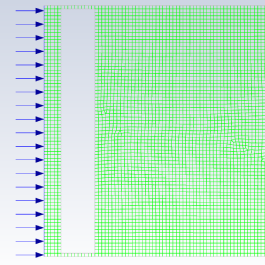
\includegraphics[width=\textwidth]{../report_assets/mesh_before_moving.png}
        \caption{Mesh at Beginning of Simulation}\label{fig:2D-tank}
    \end{minipage}
    \hfill
    \begin{minipage}{0.45\textwidth}
        \centering
        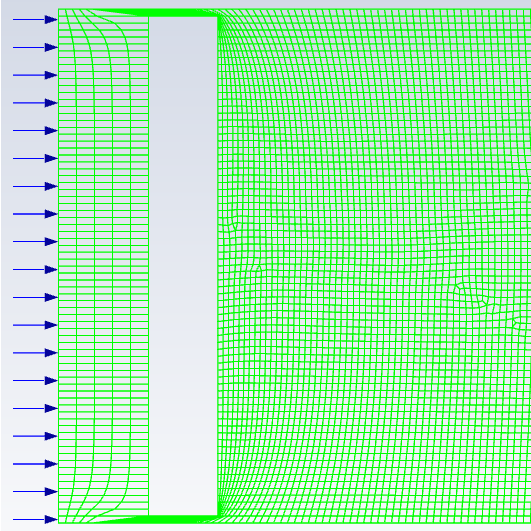
\includegraphics[width=\textwidth]{../report_assets/mesh_after_moving.png}
        \caption{Mesh at End of Simulation}\label{fig:mesh-tank}
    \end{minipage}

\end{figure}
obviously not ideal but no other option

next the simulation was ran under zero gravity as this was simpler to implement, crashing happened at different times in the simulation based on the speed of the piston so it is thought to be because of the meshing problem

when gravity was turned on the simulation crashed even faster, this is thought to be because the powder packs down to the bottom and then the piston is trying to push powder that cannot compress anymore creating physical instabilities

















% \subsection{Moving piston simulation}
% governing equations eularian-eularian
% 2d is valid because:
% 2D vs 3D Eulerian Multiphase Simulations of a Piston-Driven Fluidised Bed
% Flow Features in 2D vs 3D Multiphase Models
% Hydrodynamics and Void Distribution: Two-dimensional Eulerian-Eulerian simulations can reproduce many qualitative behaviors of fluidised beds, but they often differ quantitatively from three-dimensional models. A key issue is that 2D models tend to over-predict void fractions and bed expansion, especially at higher flow velocities
% link.springer.com
% . This occurs because neglecting the third dimension forces the gas-solid flow into a constrained plane, which exaggerates hydrodynamic structures and fluctuations
% link.springer.com
% . In practical terms, a 2D simulation may show larger void regions (bubbles) and more vigorous oscillations in solid concentration than a real 3D system would. These differences mean that certain flow features are not identical between 2D and 3D:Bubble Dynamics: Gas bubbles in a fluidised bed behave differently in a 2D domain. Studies have found that bubbles remain smaller and rise more slowly in a 2D (pseudo-2D) bed than in a full 3D bed
% witpress.com
% . In a 3D simulation or experiment, bubbles can expand and coalesce in three directions, forming larger voids that accelerate upward. The 2D constraint suppresses some coalescence, so the bed may appear “bubblier” (many small bubbles) or even form slugging bubbles that span the width. This impacts particle motion and could alter the paths through which solids circulate and exit the bed.
% Circulation and Wall Effects: Three-dimensional beds allow complex circulation patterns — particles can move around bubbles and across the entire cross-section. In a 2D model, by contrast, flow is essentially confined between two parallel walls (the front and back of the 2D slice). This artificial confinement increases wall friction effects and creates a large circulating cell in the 2D plane that has no out-of-plane escape. As a result, 2D simulations may produce stronger single circulation loops or jetting along the centerline, whereas a 3D bed would have more distributed flow paths (including around the perimeter of bubbles or toward the center of a cylinder). Such differences could influence how continuously and evenly the powder flows out — 3D systems tend to have more uniform, axisymmetric flow, while 2D systems might exhibit more pronounced channeling or periodic “puffing.”
% Turbulence and Mixing: The restriction to two dimensions also affects turbulence and mixing of the phases. Fully 3D turbulent eddies and clusters cannot form in a 2D plane, so 2D simulations often show greater oscillatory behavior (numerical instability or large-scale swings) but less of the small-scale chaotic mixing present in 3D
% link.springer.com
% . For example, pressure fluctuation spectra differ: only a 3D simulation can capture realistic pressure dynamics, whereas a 2D model gives a distorted spectrum
% witpress.com
% . This means the distribution of particles and the stability of the fluidization can differ — a 3D bed might self-buffer some fluctuations by distributing them in all directions, while a 2D bed tends to amplify fluctuations within its constrained geometry.
% Implications for Mass Flow Features: These flow-feature disparities imply that certain phenomena affecting mass outflow could differ between 2D and 3D. For instance, jetting and channeling of powder-gas mixture might be more pronounced in one case versus the other. A 3D piston-driven bed could develop a roughly axisymmetric flow of powder out of the piston region, whereas a 2D model might produce a sheet-like ejection that interacts differently with the walls. Likewise, particle distribution in 3D may be more uniform across the cross-section of an outlet, while in 2D it might be clumped or stratified, potentially affecting instantaneous mass flow rates. Overall, 2D models capture the qualitative flow patterns (e.g.fluidization regimes, general trends in circulation), but certain 3D-specific effects (like true spatial distribution of particles, or the full spectrum of bubble sizes) are lost, which can influence the accuracy of mass flow predictions
% witpress.com
% witpress.com
% . Researchers therefore caution that 2D CFD results should be used primarily for sensitivity studies or trend analysis, whereas 3D simulations are needed to accurately reproduce absolute measures like bed expansion, bubble size distributions, and pressure oscillation characteristics
% witpress.com
% witpress.com
% . In short, 2D and 3D models can differ in circulation patterns, particle clustering, wall friction effects and turbulence - all of which may affect the steady powder outflow rate.
% Linearity of Piston Velocity vs. Powder Mass Flow Rate
% Experimental Observation: In piston-driven fluidised beds (such as pneumatic powder feeders or powder-fueled engines), experiments consistently show that the powder mass flow rate increases approximately linearly with piston velocity (or with related parameters like the throttle/orifice opening)
% researchgate.net
% . Essentially, driving the piston faster injects a larger volume of gas-solids mixture per unit time, yielding a higher mass flow. This linear relationship holds as long as the system is operating below any choking or saturation limits. For example, one study of a powder fuel feeding system found a “high linear tendency” between the mass flow rate and the minimum throttle area (which correlates with piston drive conditions), within the tested range
% researchgate.net
% . Such linear scaling is a fundamental expectation for a displacement-driven flow. 2D Simulation vs 3D Reality: A well-configured 2D Eulerian-Eulerian simulation should qualitatively preserve this linear trend. If the piston (modeled perhaps as a moving wall or boundary in Fluent) is run at different velocities in a 2D model, one would observe that the outflow of powder increases proportionally. In fact, simplified models often treat the piston-induced flow like a controlled volumetric flow rate, which inherently is linear with piston speed in the absence of complex losses. The key question is accuracy: whether the 2D model’s slope of the mass flow vs. velocity curve matches that of a real 3D system. Geometric constraints can introduce some error here. For instance, 2D simulations, by overestimating void fraction and ease of fluidization, might predict slightly higher mass flow for a given piston speed than a 3D simulation or experiment would
% link.springer.com
% . This is because the 2D model may fluidize the powder bed more readily (bubbles percolating easily in the planar slice), offering less resistance to the piston. On the other hand, certain flow resistances (like friction along side walls or limitations in cross-sectional expansion) in 2D could also cause underestimation in some regimes. Notably, discrepancies are expected to grow at more extreme velocities or flow rates. Xie et al. found that when gas velocities are high, the divergence between 2D and 3D models becomes significant - 2D could not satisfactorily predict the hydrodynamics observed in a 3D cylindrical bed
% link.springer.com
% . By contrast, at lower velocities (milder fluidization), 2D and 3D results were more similar
% link.springer.com
% . Translating this to a piston-driven scenario: at modest piston speeds (near the linear operating regime), a 2D simulation will likely yield a linear mass flow response very close to reality. However, as piston velocity increases (approaching choking flow or very aggressive fluidization), the 2D model might deviate - for example, it might fail to capture the onset of non-linearity or throughput limitations that a 3D system would experience. Real 3D systems can develop complex flow distribution (e.g. some regions flowing while others channel or form stagnant zones) at high rates, whereas a 2D model may either over-homogenize this or exhibit unphysical oscillations. Thus, while the linear relationship itself is likely to appear in 2D simulations, the fidelity of its slope and any departure at extremes must be treated with caution. Validation against 3D data or correlations is advised if one plans to use 2D results for quantitative predictions of mass flow.
% Reliability of 2D Predictions and Use in Design
% Early-Stage Design Use: Despite their limitations, 2D multiphase simulations are widely used in early design and feasibility studies because they are much less computationally intensive than 3D models. Importantly, they capture the basic trends and physics of the system, which is often sufficient for preliminary performance estimates. As noted in a recent review, for certain applications like preliminary thermodynamic design or scouting different operating conditions, the more complex 3D approach “does not offer significant benefits” over 2D in terms of high-level outcomes
% link.springer.com
% . The core behaviors - e.g. how increased piston speed affects flow, or how changes in gas feed influence fluidization - are reflected reasonably well in 2D. In fact, 2D simulations can be effectively utilized to illustrate behavioral trends, albeit with some “acceptable disadvantages” such as misrepresentation of exact bed expansion
% link.springer.com
% . In the context of a piston-driven powder bed, a 2D Fluent model would be a theoretically sound and practically convenient tool to predict whether, say, doubling the piston velocity doubles the powder delivery rate (and it likely will show that linear doubling trend). This helps an engineer get a quick sense of performance scaling without the overhead of a full 3D simulation. Known Limitations: However, one should not take 2D results as gospel when it comes to absolute performance or detailed flow behavior. Multiple validation studies have concluded that 2D simulations should be used with caution and primarily for qualitative insight or sensitivity analysis
% witpress.com
% witpress.com
% . They are not fully predictive of 3D behavior in a quantitative sense. For example, a 2D model might predict a certain mass flow rate for a given piston speed that differs from the real 3D value by a noticeable margin (due to differences in void fraction and wall friction effects). It might also fail to predict phenomena like unequal powder distribution in a 3D hopper, or the exact point where increasing piston velocity no longer yields proportional increases (onset of choking). As one study put it, only a 3D simulation was able to reproduce both the correct bed height and the dynamic pressure fluctuations of a bubbling bed, whereas 2D had significant deviations
% witpress.com
% . Conclusion - “Acceptable with Caution”: For the piston-driven fluidised bed scenario, using a 2D Eulerian-Eulerian Fluent simulation is reasonable in the early project stages. It offers a fast and informative approximation, and it will likely correctly indicate that there is a linear relationship between piston speed and powder mass flow under normal operating conditions. This makes it a practically acceptable tool for initial design and performance prediction. The literature supports this usage: 2D models can reliably rank design options and reveal trends (e.g. that higher piston speeds yield proportionally higher flow)
% researchgate.net
% , and they can guide engineers on what range of operation is plausible. The theoretical basis (continuity and momentum balance of two-phase flow) is sound, so there is no fundamental reason the 2D model would invert or lose the linear trend. What must be kept in mind is that extrapolating 2D results to 3D comes with uncertainty. Engineers should apply conservative corrections or eventually verify with a 3D model or experiments. In early design, one might use 2D to narrow the design space (thanks to its speed), then use a higher-fidelity 3D simulation on the shortlisted cases. By doing so, one benefits from the strengths of both approaches. In summary, 2D Eulerian-Eulerian simulations are theoretically sound for capturing the essential flow physics and trends of a piston-driven powder bed, and they are practically very useful in the initial design phase. They do preserve the linear piston velocity vs. mass flow relationship observed in 3D
% researchgate.net
% . Yet, because of geometric constraints, they can introduce errors in flow details and magnitudes, so their predictions should be regarded as preliminary. For final design confidence - especially if subtle 3D flow features (circulation patterns, non-uniform outflow, etc.) matter - a 3D simulation or experimental validation is recommended
% witpress.com
% link.springer.com
% . The consensus in the literature is that 2D and 3D approaches complement each other: use 2D for efficiency and scoping, and 3D for accuracy and final verification
% link.springer.com
% witpress.com
% . Sources: Recent computational studies and reviews of fluidised bed modeling and pneumatic powder feeding have informed these conclusions. Notably, comparisons by Yılmaz et al. (2025) on 2D vs 3D fluidised bed reactors highlight where 2D falls short and where it suffices
% link.springer.com
% link.springer.com
% . Similarly, Cardoso et al. (2019) and Xie et al. have demonstrated the specific differences in bed expansion, bubble motion, and pressure dynamics between 2D and 3D models
% witpress.com
% witpress.com
% . Experimental research on piston-driven powder feeders provides the empirical evidence of linear flow scaling and helps validate the trends seen in simulations
% researchgate.net
% . All these studies collectively suggest that a 2D Eulerian-Eulerian Fluent simulation is a useful predictive tool with known limitations, and with careful interpretation it can be reliably used to inform 3D behavior in the early stages of engineering design. The linear piston velocity-mass flow relationship is expected to appear in the 2D model (as observed experimentally), but final design decisions should account for 3D effects identified in the literature.
% solver settings
% geometry and mesh details
% boundary and initial conditions